\section{Проектирование синхронного фреймворка}

Один из основных подходов, используемых при разработке платформы 
– это максимальная гибкость и расширяемость. В платформе 
используется абстракция – механизм, который является 
классом-оберткой вокруг потоконебезопасного класса и решает 
определенную задачу синхронизации внутри платформы. При желании, 
разработчик, использующий платформу для своих задач  может 
использовать как готовые механизмы, так и может добавлять свои 
механизмы, если считает, что они ему не подходят, расширяя тем 
самым функционал платформы.

Продемонстрировать гибкость платформы можно наглядно на 
следующем примере: в платформе есть механизм, ответственный за 
запуск и исполнение всех модулей в системе; есть несколько 
вариантов этого механизма – обычный линейный, многопоточный, 
многопоточный с использованием пула потоков. При использовании 
системы на различных процессорах – одноядерных или многоядерных 
имеет смысл использовать различные режимы исполнения 
соответственно, чтобы исключить затраты на лишнюю синхронизацию 
и обеспечить максимальную производительность. Так, например, нет 
смысла запускать многопоточный режим на старом одноядерном 
процессоре, и, в ту же очередь, нет смысла не использовать 
возможность распараллеливания на многоядерных процессорах. 
Гибкость и расширяемость описываемой платформы позволяет 
подстроить ее под необходимую среду, в которой ей придется 
работать.

В данной реализации под механизмами будет подразумеваться класс-обертка вокруг потоконебезопасного класса, которая инкапсулирует все вызовы к данному классу в функциональный объект и помещает его в потокобезопасную очередь. Использование механизма отложенных синхронизаций позволяет избавиться от проблем зацикливания при ситуации, например, когда какой-нибудь модуль отправляет сообщения сам себе. Также, позволяет с легкостью подобрать нужную реализацию очереди под конкретную ситуацию. В асинхронной версии библиотеки структура механизма отличается от описанной в данном разделе.

На рис. \ref{im:2_2_1_sync}, представлена схема синхронного прототипа ядра системы. Данная диаграмма классов включает только основной набор классов, которые демонстрируют механику взаимодействия между отдельными компонентами системы:

\begin{figure}[h]
    \centering{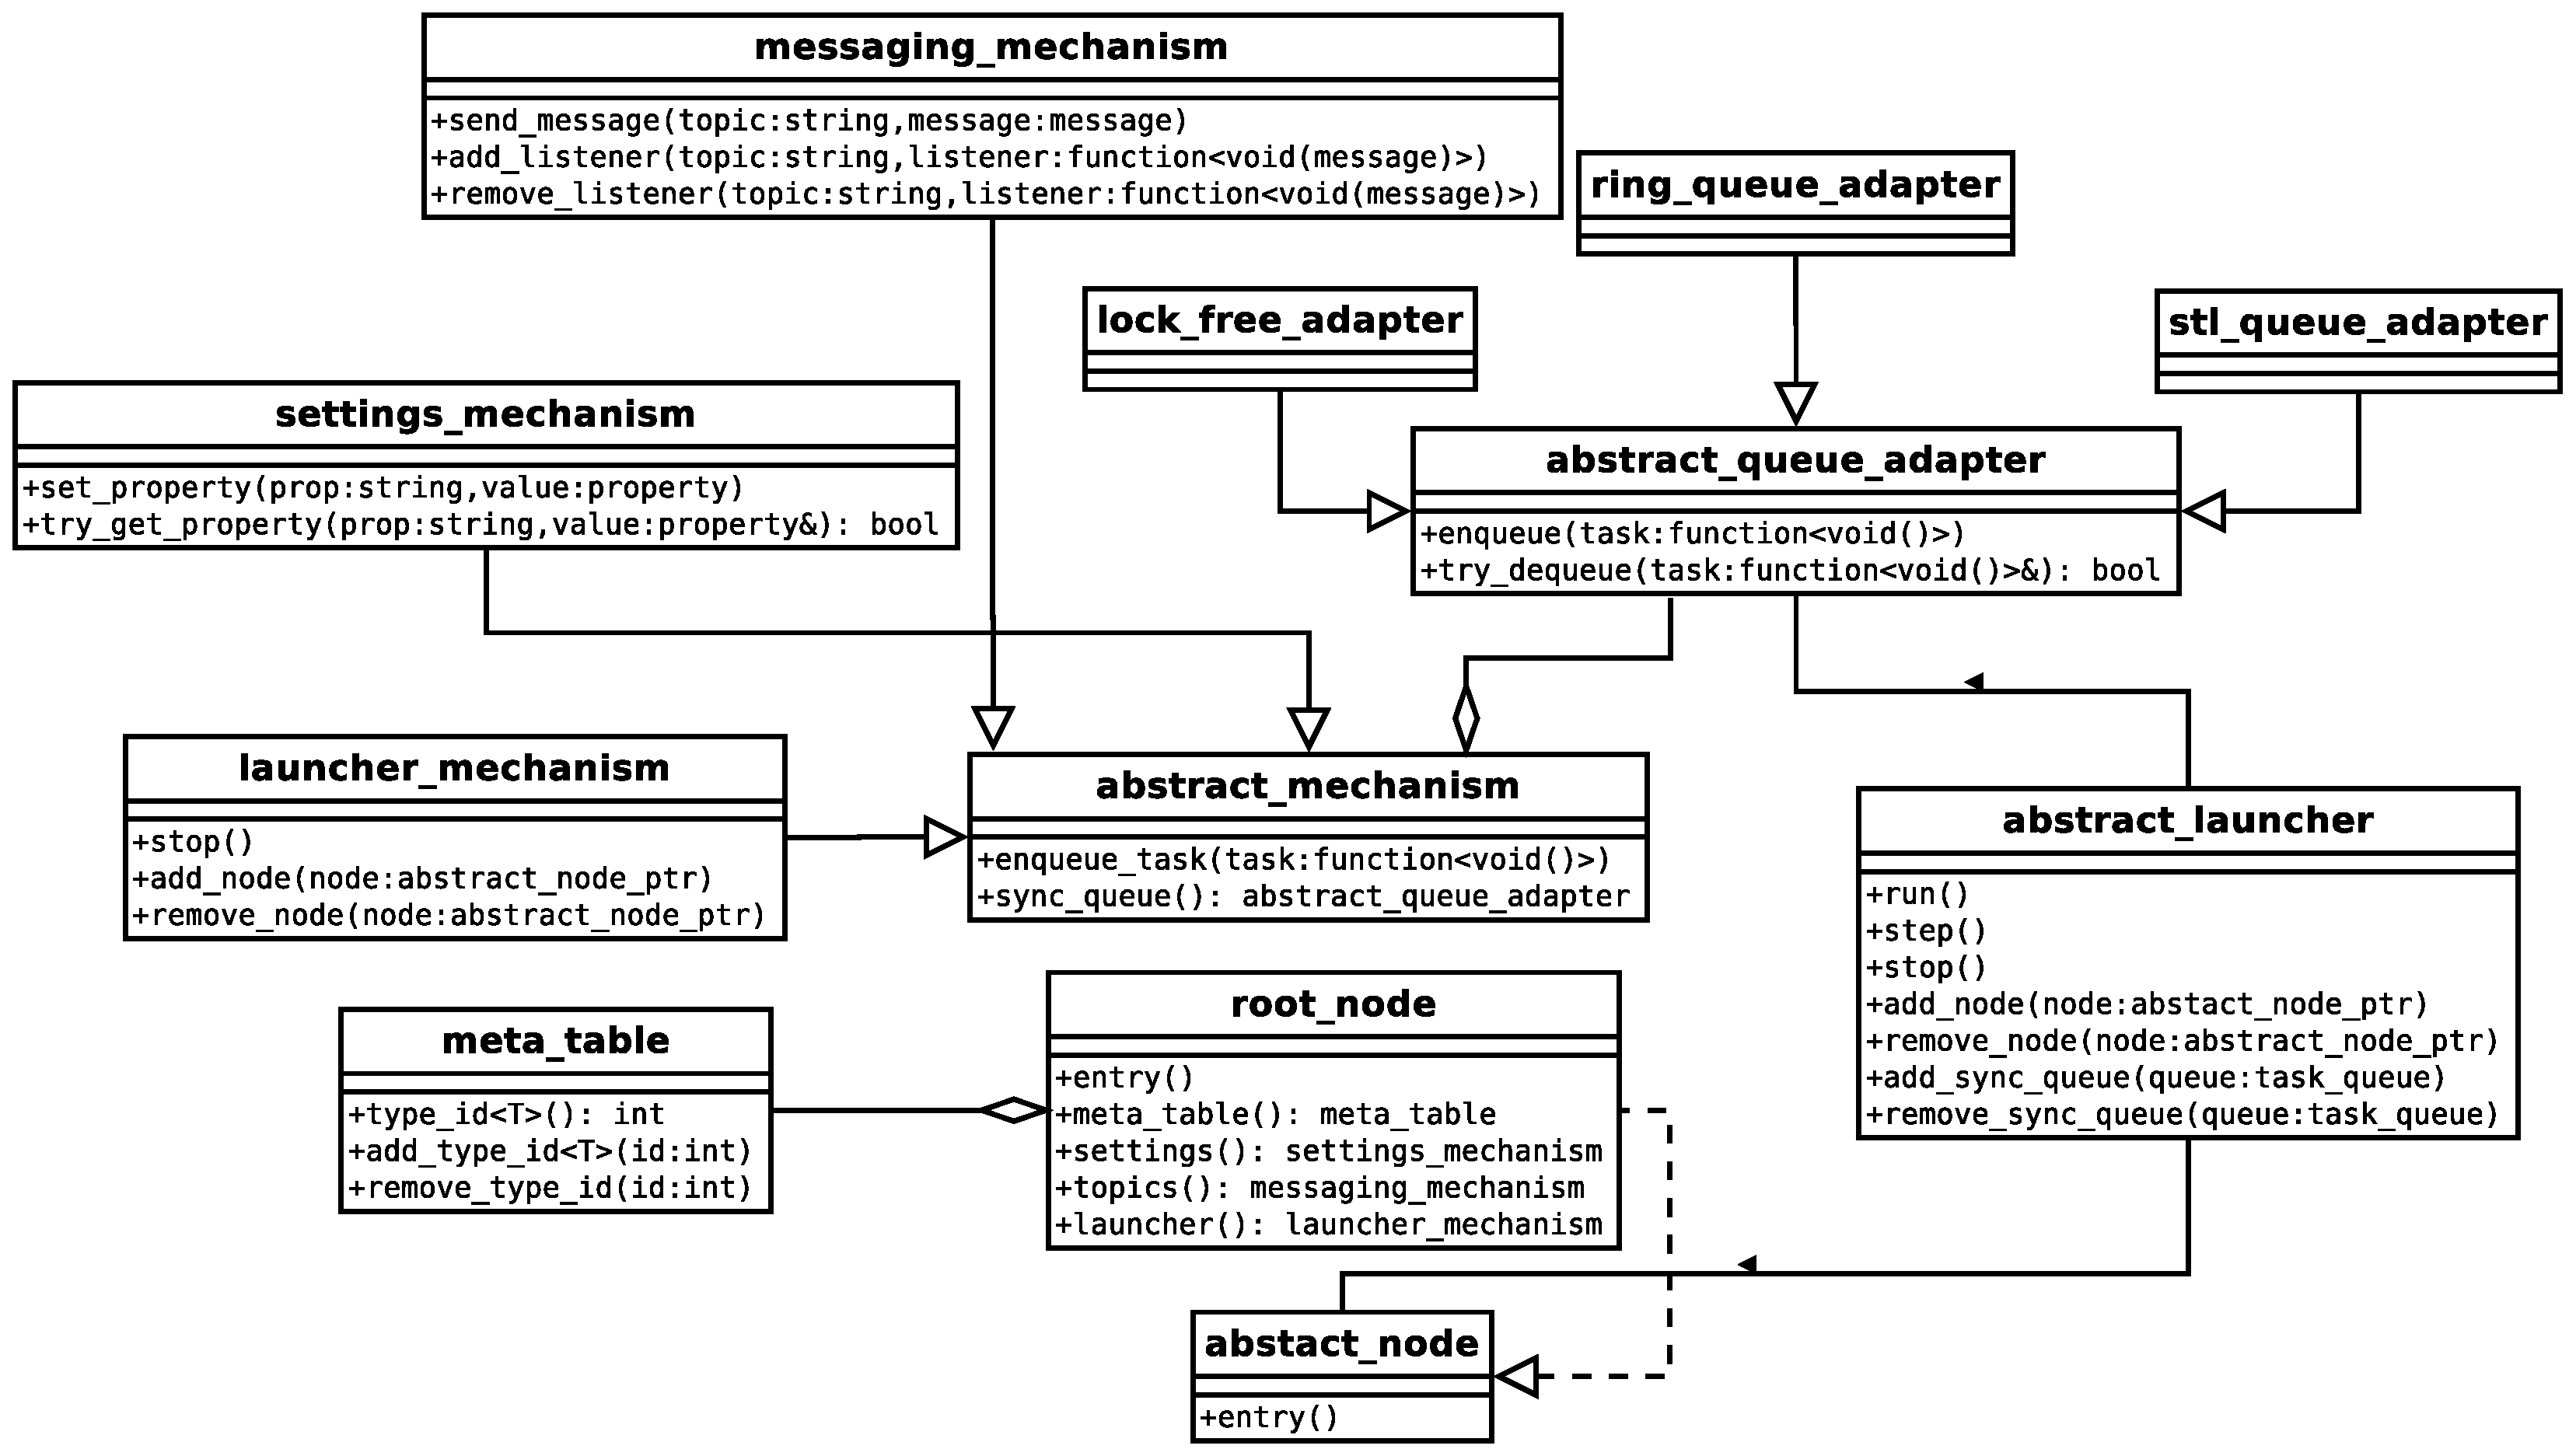
\includegraphics[width=1\linewidth]{2_2_1_sync}}
    \caption{Диаграмма классов синхронной версии фреймворка}
    \label{im:2_2_1_sync}
\end{figure}

\textit{abstract\_launcher} --- интерфейс исполняющего класса. Реализация данного класса должна хранить указатели на модули и очереди синхронизаций и обеспечивать требуемый порядок исполнения, например, последовательно в одном потоке или с использованием пула потоков.

\textit{abstract\_queue\_adapter} --- интерфейс компонента, 
необходимого для обеспечения отложенной синхронизации. Он 
передает все задачи по синхронизации на определенные очереди. 
Адаптер предоставляет единый интерфейс для добавления 
и получения элементов из очереди.

\textit{stl\_queue\_adapter} --- компонент, необходимый для работы с очередью из стандартной библиотеки C++ STL. В данном классе не используются блокировки для повышения производительности на одноядерных системах.

\textit{lock\_free\_adapter} --- компонент, необходимый для 
работы с lock-free(без использования мьютексов) очередью. В 
проекте используется реализация очереди Камерона Десрочерза.

\textit{ring\_queue\_adapter} --- компонент, необходимый для работы с  циклической очередью фиксированного размера.

\textit{abstract\_node} --- интерфейс, позволяющий создавать 
независимые компоненты системы --- модули, каждый из которых 
может быть ответственен за свой конкретный функционал. Модули 
<<не знают>> о существовании других модулей, то есть они на 
самом деле полностью независимы друг от друга, их взаимодействие 
и исполнение обеспечено ядром системы. Такой подход к созданию 
этой абстракции также позволяет переиспользовать разработанные 
на ее основе модули при различных конфигурациях описываемой 
робототехнической платформы, а также позволяет исполнять каждый 
модуль в отдельном потоке без дополнительных затрат 
процессорного времени на синхронизацию. 

\textit{abstract\_mechanism} --- абстрактный класс для компонентов системы, обеспечивающих какой-либо потокобезопасный вид взаимодействия между модулями и с ядром системы. Класс содержит потокобезопасную очередь функциональных объектов, куда помещаются все вызовы к базовому классу. Для функционирования механизма Указатель на очередь должен быть зарегистрирован в экземпляре класса abstract\_launcher.

\textit{launcher\_mechanism} --- компонент, реализующий интерфейс abstract\_mechanism, обеспечивающий взаимодействий с конкретной реализацией abstarct\_launcher, позволяет добавлять и удалять модули, запускать и останавливать систему.

\textit{messaging\_mechanism} --- компонент, реализующий интерфейс abstract\_mechanism, обеспечивающий возможность коммуникации и обмена данными между модулями путем отправки сообщений. Данный механизм реализован с использованием паттерна <<издатель-подписчик>>. Экземпляр <<слушателя>> добавляется в список к именованному <<топику>>, куда в дальнейшем любой модуль может отправлять сообщения. Данный механизм реализован по аналогии с системой рассылки сообщений в ROS.

\textit{services\_mechanism} --- компонент, реализующий 
интерфейс abstract\_mechanism, обеспечивающий возможность 
запуска требуемых методов по их имени. Вызовы происходят в 
неблокирующем режиме, поэтому система позволяет отправить 
несколько запросов до получения ответа. Аргументы метода 
передаются в структуре сообщения. Результат выполнения будет 
записан в объект результата после выполнения функции. 

\textit{meta\_table} --- класс, который содержит информацию для идентификации сообщений. В данной реализации использовалась библиотека google protocol buffers. Поскольку в данной библиотеке используется не тривиальный алгоритм сериализации и десериализации, сообщения внутри системы передаются в <<сыром>> виде для уменьшения дополнительных нагрузок на систему. При регистрации нового типа сообщений так же создается экземпляр <<абстрактной фабрики>> для сообщений, который позволяет при получении сериализированных данных верифицировать их и создать экземпляр сообщения.

Следует так же уделить внимание классу сообщений 
\textit{message}. В данной реализации, как было сказано ранее, 
используется библиотке google protocol buffers для генерации 
сериализируемых сообщений. Сериализация необходима, например, 
для передачи сообщения через сетевой протокол. Сообщения 
хранятся и передаются внутри системы через умные указатели 
(\textit{std::shared\_pointer}) на экземпляр структуры, которая 
хранит данные. Данный прием позволяет передавать сообщения 
внутри системы без дополнительных затрат на копирование данных, 
а так же автоматически освобождать занятые ресурсы памяти, что 
дает существенный прирост в производительности всей системы при 
рассылке сообщений нескольким <<слушателям>>.

При проектировании в дальнейшем было принято решение отказаться 
от реализации системы сообщений с использованием мета-таблиц и 
google protocol buffers. Данное решение позволяет использовать 
контейнеры сообщений без десериализации, но накладывает 
ограничения на систему при коммуникации с удаленными агентами 
системы. Так же по этой причине система предполагает, что модули 
используют ограниченный фиксированный набор сообщений, которые 
предварительно уже зарегистрированы в системе, что существенно 
снижает возможность расширять систему и использовать в модулях 
<<не стандартные>> сообщения.

По умолчанию в системе реализован класс 
\textit{abstract\_launcher}, который поочередно запускает 
обработку модулей и стадию синхронизации. Такой порядок 
исполнения позволяет исключить гонку за данные при многопоточном 
исполнении, а следовательно упростить структуру модулей в 
случае, если модуль не создает собственного потока исполнения. 
Далее в этом разделе будет подробнее описываться данный способ 
обеспечения потокобезопасности.

\begin{figure}[h]
    \centering{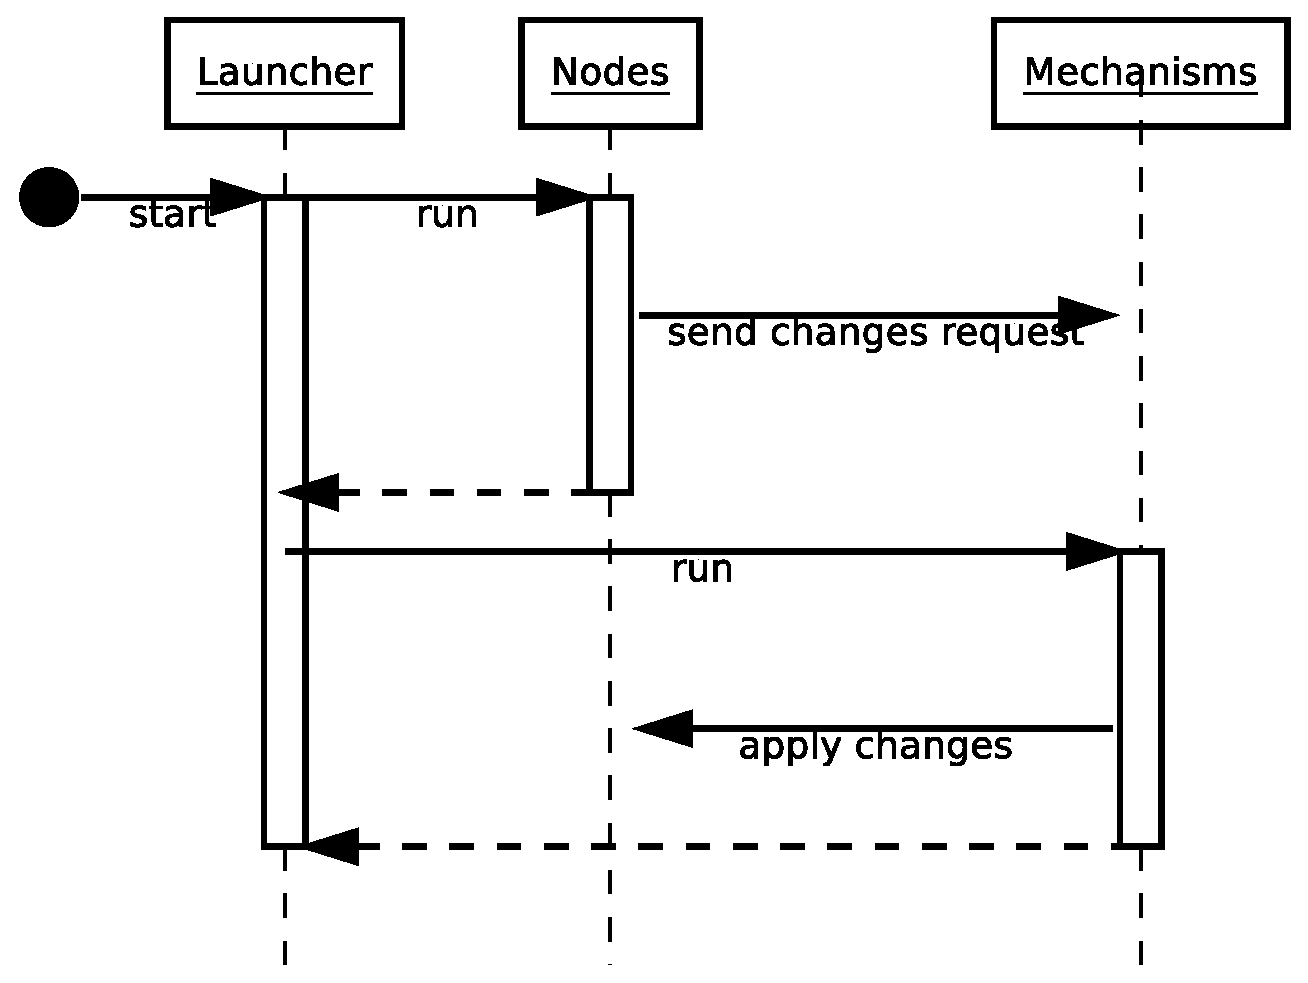
\includegraphics[width=0.7\linewidth]{2_2_2_sequence_diag}}
    \caption{Принцип работы класса \textit{abstract\_launcher}}
    \label{im:2_2_2_sequence_diag}
\end{figure}

На рис. \ref{im:2_2_2_sequence_diag} представлена диаграмма 
последовательностей, в которой изображен сценарий коммуникации 
модулей с ядром системы (механизмами синхронизации). В данном 
графике продемонстрирована одна итерация обработки событий в 
системе. Сначала группа модулей передает требуемые запросы 
механизмам синхронизации. По завершении обработки модулей 
начинается обработка запросов механизмов, которые возвращают 
результаты нодам.

Реализация механизмов синхронизации является ключевым звеном в разработке архитектуры данного фреймворка. Предполагается, что система работает в рамках одного адресного пространства и отдельные компоненты могут исполняться в отдельных потоках. Поскольку механизмы являются средством взаимодействия между модулями также предполагается, что количество обращений к данным классам достаточно высоко и поэтому блокирующий вызов может существенно понизить отклик всей системы. Блокирующий вызов допустим для методов с низкой вероятностью возникновения ситуации гонки за данные.

\begin{figure}[h]
    \centering{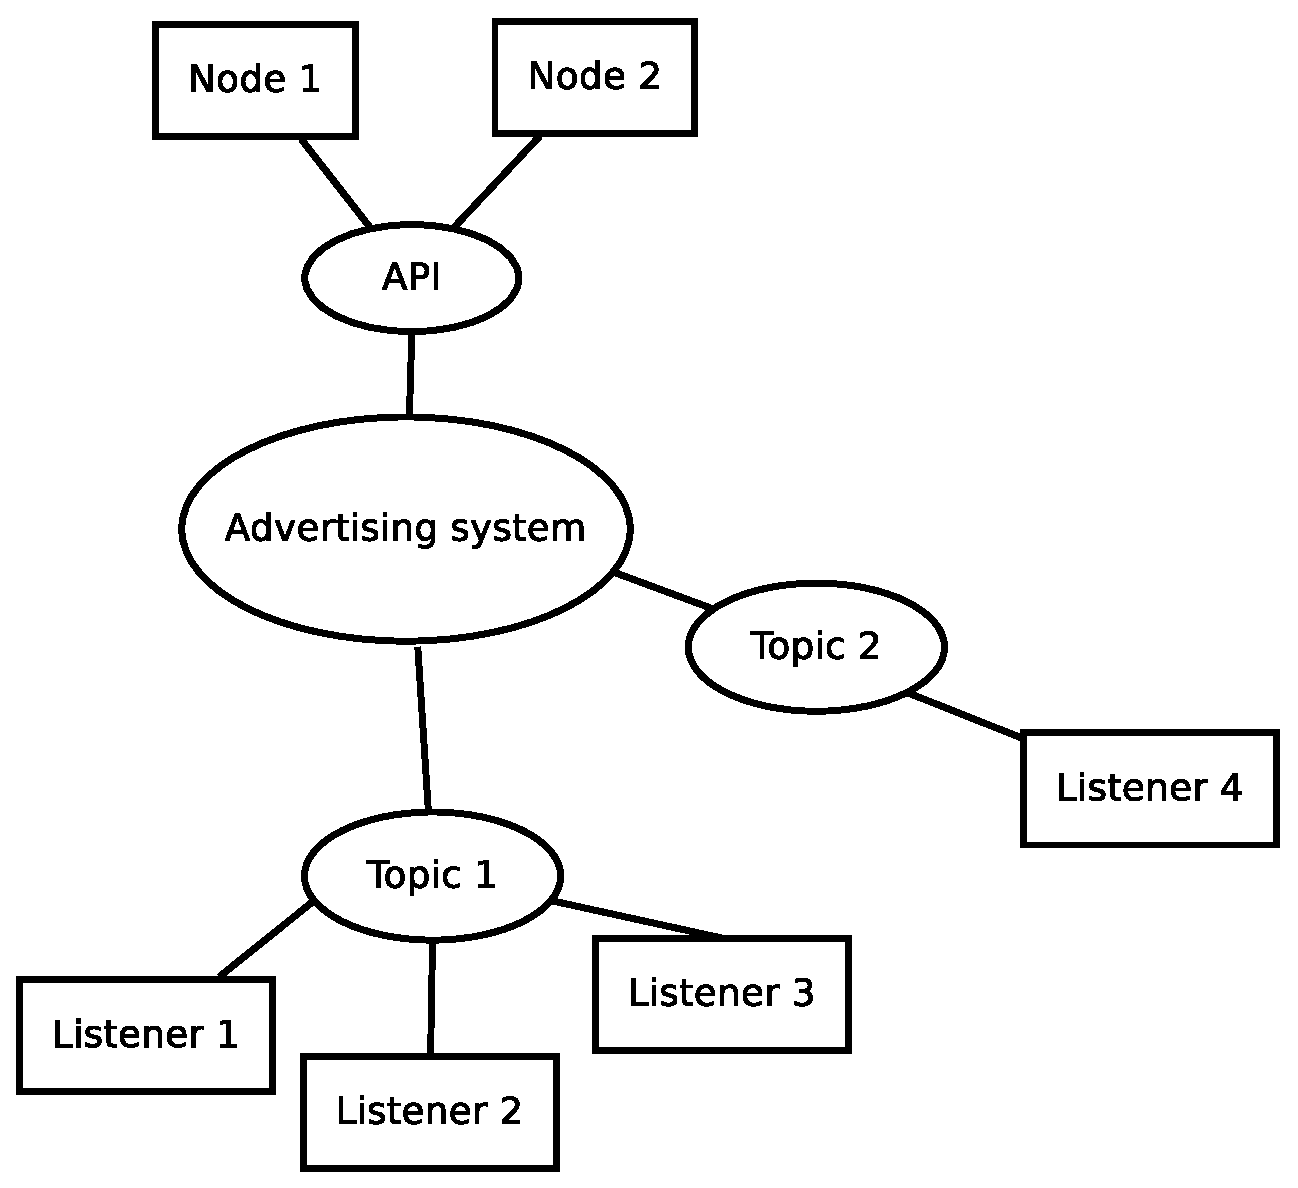
\includegraphics[width=0.7\linewidth]{2_2_3_topic}}
    \caption{Система рассылки сообщений}
    \label{im:2_2_3_topic}
\end{figure}

На рис. \ref{im:2_2_3_topic} схематически изображен граф системы 
рассылки сообщений с двумя модулями, двумя топиками и четырьмя 
слушателями. На данном графике <<механизм>> выступает в роли 
\textit{API} доступа к системе рассылки. Ребра графа показывают 
наличие прямого доступа к компоненту: например \textit{node 1} и 
\textit{node 2} могут обращаться к \textit{API} (application 
programming interface, программный интерфейс приложения) 
напрямую, но не могут взаимодействовать с \textit{advertising 
system}. Круглые вершины обозначают компонент ядра системы, а 
прямоугольные --- компоненты, реализованные пользователем.

Интерфейс системы рассылки сообщений включает в себя четыре функции: отправить сообщение в топик, получить список топиков, добавить слушателя сообщений в топик и удалить слушателя из топика. Механизм дублирует функции системы рассылки. Топик может существовать только если у него есть хотя бы один подписчик --- это требуется для освобождения памяти при удалении подписчиков. Предполагается, что добавление и удаление слушателей может осуществляться с применением блокирующей синхронизации, т.к. эта операция не должна вызываться с высокой частотой.

Топик является контейнером для подписчиков и позволяет проверить наличие у него слушателей, добавить нового слушателя, удалить слушателя и разослать сообщение всем слушателям.

Далее рассмотрены различные варианты взаимодействия модулей с 
механизмом синхронизации на примере данной структуры в ситуации, 
когда модули обрабатываются параллельно. В данном анализе будут 
рассмотрены возможные способы обеспечения потокобезопасности 
механизма. По этому принципу устроены другие механизмы 
синхронизации в системе. В блок-схемах, изображенных ниже, 
представлен только набор ключевых действий и проверок, которые 
выполняются в алгоритме. 

\begin{figure}[h]
	\centering{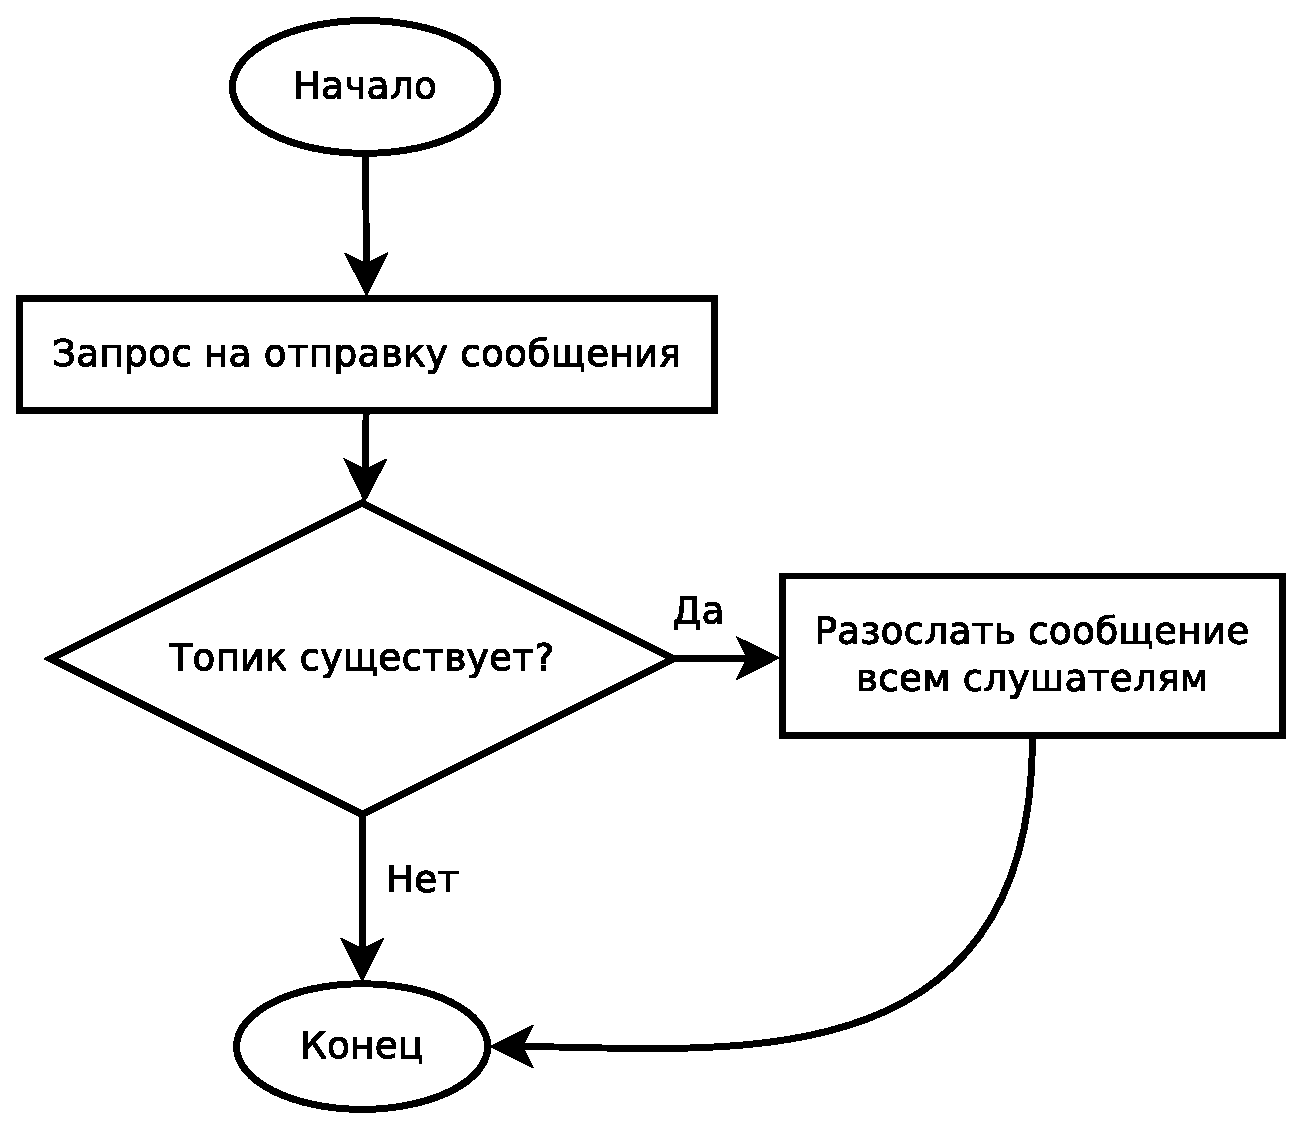
\includegraphics[width=0.6\linewidth]{2_2_5_send_message}}
	\caption{Алгоритм отправки сообщения}
	\label{im:2_2_5_send_message}
\end{figure}

На рис. \ref{im:2_2_5_send_message} изображена блок-схема алгоритма отправки сообщения. Из схемы видно, что после отправки запроса выполняется проверка на существование топика, только после чего выполняется рассылка сообщений в данный топик. При одновременном исполнении данной последовательности  действий возникает две возможные ситуации гонок за данные:

\begin{itemize}  
	\item топик был удален во время проверки на его существование;
	\item топик был удален во время рассылки сообщений;
	\item изменен набор слушателей в топике во время рассылки сообщений.
\end{itemize}

\begin{figure}[h]
	\centering{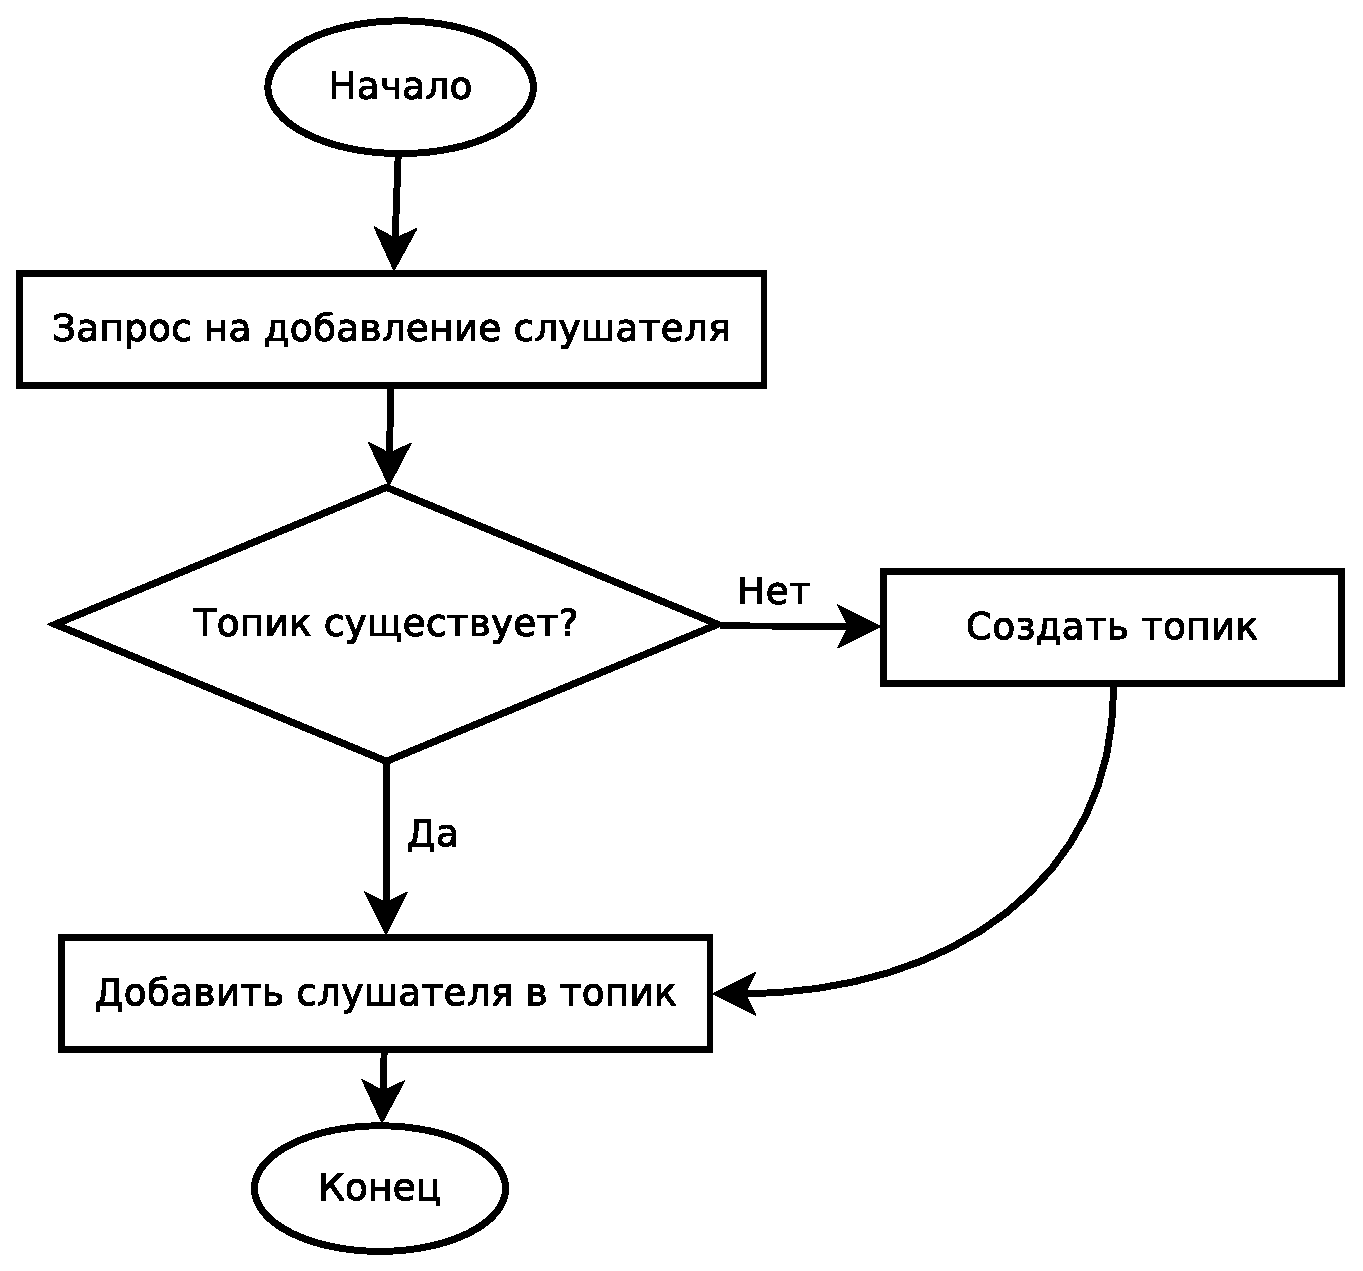
\includegraphics[width=0.6\linewidth]{2_2_4_add_listener}}
	\caption{Алгоритм добавления слушателя}
	\label{im:2_2_4_add_listener}
\end{figure}


На рис. \ref{im:2_2_4_add_listener} изображена блок-схема последовательности действий для добавления нового слушателя в топик. Здесь, как и в случае с рассылкой сообщений, возникают схожие ситуации:

\begin{itemize}  
	\item топик был удален во время проверки на его существование;
	\item топик был удален во время добавления слушателя в топик;
	\item изменен набор слушателей в топике во время добавления;
	\item топик мог быть создан другим потоком во время его создания в текущем;
	\item изменен набор слушателей в топике во время добавления.
\end{itemize}

\begin{figure}[h]
	\centering{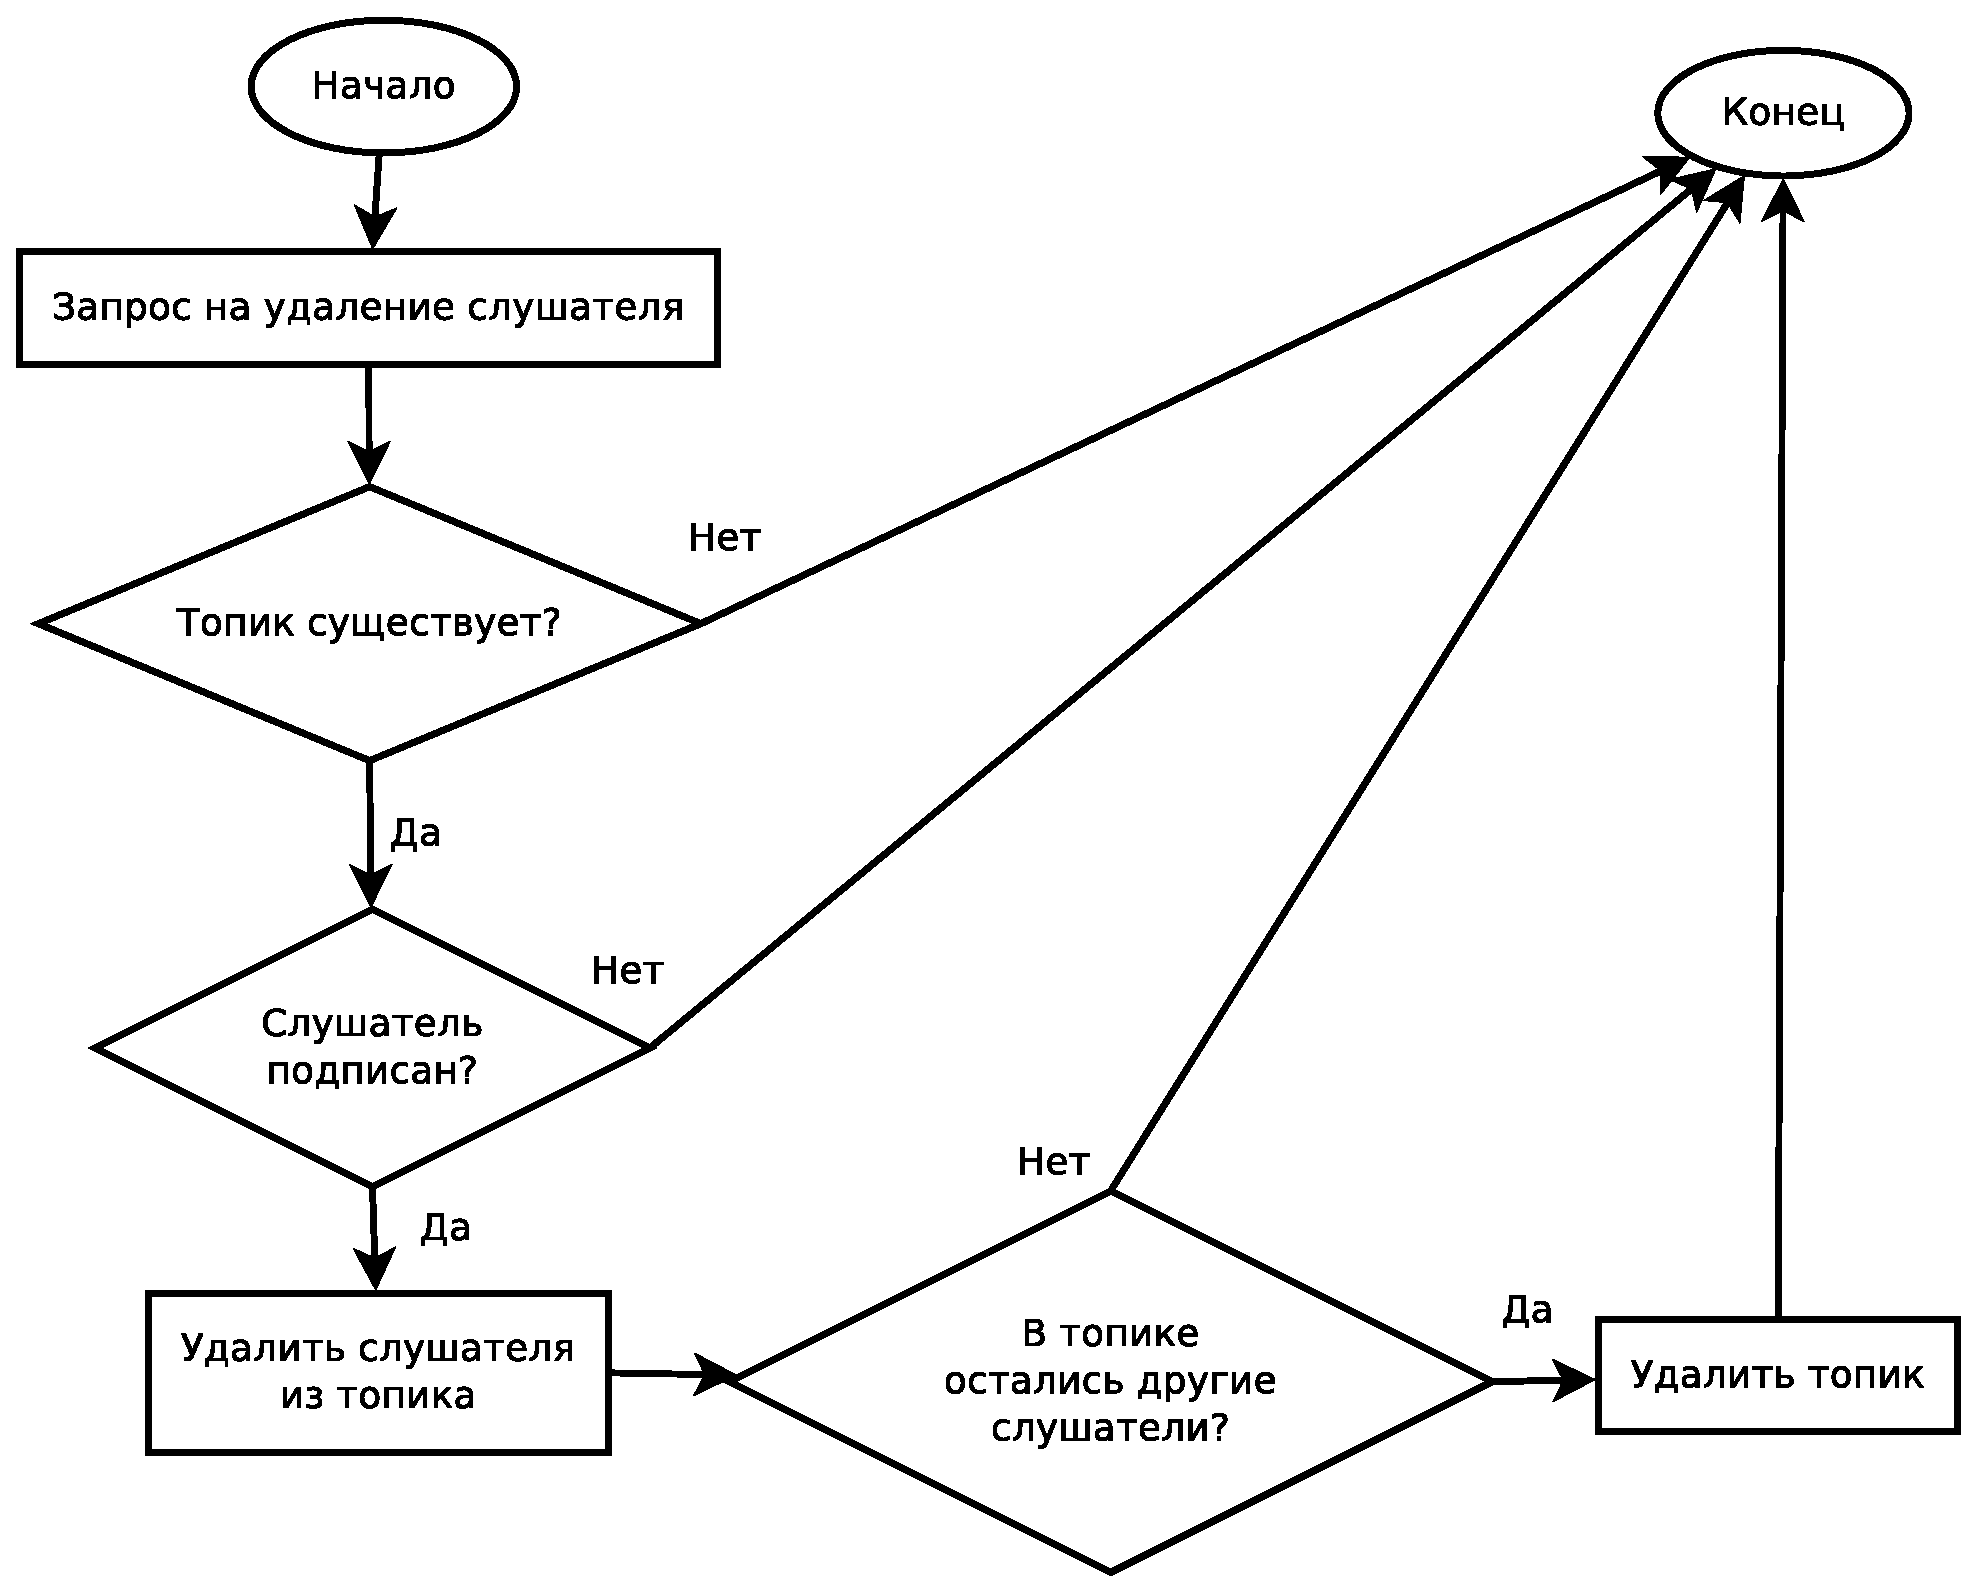
\includegraphics[width=0.8\linewidth]{2_2_6_remove_listener}}
	\caption{Алгоритм удаления слушателя}
	\label{im:2_2_6_remove_listener}
\end{figure}

На рис. \ref{im:2_2_6_remove_listener} изображена блок-схема последовательности действий для удаления слушателя из топика. В данной последовательности возникают следующие ситуаций, где может возникнуть гонка между потоками:

\begin{itemize}
	\item изменен набор слушателей в топике во время удаления слушателя;
	\item добавлен слушатель в топик после проверки на наличие других слушателей;
	\item изменен набор слушателей в топике во время удаления топика.
\end{itemize}

Во время получения списка существующих топиков возможна только одна ситуация гонки: были добавлены или удалены топики во время их перечисления.

В случае с использованием алгоритмов без блокировок можно 
обеспечить потокобезопасность системы рассылки с применением 
очереди функциональных объектов, которая позволит упорядочить 
вызовы из разных потоков в одну последовательность. 
Потокобезопасные хэш-таблицы или списки без блокировок 
позволяют обеспечить безопасность только в операциях с 
контейнером и исключит ситуацию гонки только в некоторой части 
из возможных случаев. 

Использование очереди без блокировок имеет один нюанс: операции, 
добавленные в очередь не должны быть зависимы как от состояния, 
в котором находится потоконебезопасный класс, так и друг от 
друга. Например, при исполнении отправки сообщения в топик нужно 
убедиться, что этот топик все еще существует, т.к. он мог быть 
удален с момента добавления этой операции в очередь. Все 
топики хранятся в хэш таблице и считается, что поиск элемента 
происходит за O(1) с небольшой константной задержкой.

В данном прототипе системы существует возможность исполнять параллельно в нескольких потоках задачи из стадии синхронизации и отдельно модули при гарантии, что во время синхронизации модули обрабатываться не будут. Данное свойство достигается за счет того, что во механизмы синхронизации не взаимодействуют друг с другом через прямые вызовы, как и модули.

Так же обращение из модулей к полям класса на чтение (например 
операция получения списка топиков) будет гарантированно 
потокобезопасной только в том случае, если во время этого 
обращения не обрабатывается очередь задач данного механизма. Это 
обуславливается тем, что операция чтения без блокировки 
безопасна только в том случае, если операции, изменяющие 
состояние объекта, происходят атомарно  или в случае, если 
объект неизменяем \cite{williams2012c++}.

% Ссылочка!
Как правило, очереди без блокировок работают немного медленнее, 
чем обычные однопоточные очереди с быстрым аллокатором, из-за 
синхронизации между ядрами процессора при атомарных операциях. 
Если исполнительный класс, который выполняют межмодульную 
синхронизацию, работает в одном потоке с исполняемым на данный 
момент модулем, то можно использовать отдельную обычную очередь 
для данного потока. В данной работе используется реализация 
очереди с производительностью не ниже, чем из стандартной 
библиотеки C++, поэтому эта оптимизация не была использована при 
проектировании.

% Блокирующая
Кроме того, была спроектирована система рассылки сообщений с 
блокировками для функций добавления, удаления и получения списка 
слушателей с мелкогранулярными блокировками при отправке 
сообщений.

В данной реализации список топиков и слушателей изменяется в блокирующем режиме. Список топиков имеет глобальный мьютекс для потокобезопасного обращения к нему. Каждый топик должен хранить список как слушателей, так и издателей, которые могут отправлять сообщения. Добавление в систему издателей позволят обращаться к списку слушателей напрямую, минуя глобальную хэш-таблицу, что позволит рассылать сообщения с мелкогранулярными блокировками, что в свою очередь позволяет снизить вероятность захвата одной критической секции двумя потоками.

В такой системе у каждого компонента должен быть своя локальная критическая секция: у издателя, у топика и у слушателя.

Операцию добавления слушателей можно описать следующим порядком действий:

\begin{enumerate}
	\item Захватить глобальный мьютекс хэш-таблицы и найти в ней требуемый топик.
	\item Если топик не существует, то создать его, и добавить его в хэш. В данном случае никто больше не может работать с хранилищем и поэтому данная операция потокобезопасна.
	\item Захватить мьютекс для топика. Поскольку все дальнейшие операции производятся только с данным топиком и его никто не может изменять, т.к. его локальный мьютекс заблокирован, то можно освободить критическую секцию хэш-таблицы, но при этом топик должен храниться в потокобезопасном указателе на случай, если будет пересчитан хэш после другой операции над словарем.
	\item Добавить указатель на слушателя в список слушателей топика.
	\item Для каждого издателя заблокировать его список слушателей, добавить указатель на слушателя, после чего освободить критическую секцию издателя.
	\item Освободить критическую секцию топика.
\end{enumerate}

Схожим образом в систему добавляется издатель:

\begin{enumerate}
	\item Захватить глобальный мьютекс хэш-таблицы и найти в ней требуемый топик.
	\item Если топик не существует, то создать его, и добавить его в хэш.
	\item Захватить мьютекс для топика и освободить критическую секцию хэш-таблицы.
	\item Добавить указатель на издателя в список издателей топика.
	\item Скопировать список слушателей из топика в список издателя.
	\item Освободить критическую секцию топика.
\end{enumerate}

В данной системе каждый издатель имеет свою локальную копию указателей на слушателей. Это позволяет не обращаться к глобальной хэш-таблице каждый раз, когда требуется отправить сообщение. Слушателям необязательно знать о том, откуда им будут приходить сообщения. Для удаления слушателя можно воспользоваться списком издателей, который хранится в топике.

Мелкогранулярные блокировки позволяют уменьшить время захвата глобального мьютекса, что в свою очередь оптимизирует время обращения к другим топикам из других потоков.

Отправка сообщения через издателя работает путем захвата его 
локального мьютекса, чтобы в этот момент никто не мог изменить 
его список слушателей и поочередно критических секций каждого 
слушателя при отправке сообщения. Поскольку слушатель может быть 
подписан на несколько топиков, то его нужно блокировать. 
Поскольку это единственный случай, когда нужно блокировать 
слушателей, то здесь не возникает ситуации взаимоблокировки 
(dead-lock). Также в слушателе можно использовать очередь с 
неблокирующей синхронизацией, что исключит критическую секцию 
вообще.

Удаление слушателей происходит в следующем порядке:

\begin{enumerate}
	\item Захватить глобальный мьютекс хэш-таблицы и найти в ней требуемый топик.
	\item Если топик не существует, то вернуть результат ошибки.
	\item Захватить мьютекс для топика.
	\item Если в топике нет издателей и единственный слушатель, то удалить топик из хэш таблицы и вернуть результат успеха операции, освободив все мьютексы.
	\item В противном случае освободить критическую секцию хэш таблицы.
	\item Для каждого издателя заблокировать его список слушателей, удалить указатель на слушателя, после чего освободить критическую секцию издателя.
	\item Освободить критическую секцию топика.
\end{enumerate}

Из данного списка следует выделить пункт с удалением топика. Топик удаляется только в том случае, когда на него нет ни подписчиков, ни издателей. В данном случае, когда остается только один слушатель, топик можно удалять, т.к. слушателей у него после данной операции не будет.

Удаление издателя происходит по следующему алгоритму:

\begin{enumerate}
	\item Захватить глобальный мьютекс хэш-таблицы и найти в ней требуемый топик.
	\item Если топик не существует, то вернуть результат ошибки.
	\item Захватить мьютекс для топика.
	\item Если в топике нет слушатель и единственный издатель, то удалить топик из хэш-таблицы и вернуть результат успеха операции, освободив все мьютексы.
	\item В противном случае освободить критическую секцию хэш-таблицы.
	\item Удалить издателя из списка топика, удалить из списка издателя.
	\item Освободить критическую секцию топика.
\end{enumerate}

Данная реализация исключает все описанные ранее случаи гонки за данные и использует достаточно простую архитектуру. Исполнение модулей в таком подходе может происходить без дополнительной фазы синхронизации, что существенно упрощает архитектуру исполнительного класса.

Описанный алгоритм с блокировками имеет схожу реализацию с системой сигналов-слотов в библиотеке Qt и Boost Signals2 \cite{schaling2011boost}. В дальнейшем при тестировании производительности реализации системы без блокировок и с блокировками использовалась реализация из библиотеки Boost Signals2.

